\chapter{Graphical user interface}\label{chapGUI}

This chapter introduces our graphical user interface (GUI) for conducting Bayesian regression analysis in a user-friendly environment, requiring no programming skills (drag and drop). Our GUI is built as an interactive web application using \textit{shiny} \cite{Chang2018} and incorporates packages such as \textit{MCMCpack} \cite{Martin2018} and \textit{bayesm} \cite{Rossi2017} from the \textbf{R} software \cite{R2023}. It is designed for teaching and applied purposes at an introductory level. In the following chapters of the second part of this book, we present several applications that demonstrate the potential of our GUI for applied researchers and practitioners.

\section{Introduction}\label{secGUI1}

Our GUI enables users to perform inference using Bayesian regression analysis without requiring programming skills. The latter is often a significant impediment to the widespread adoption of the Bayesian framework \cite{Woodward2005,Karabatsos2016}.

Several other graphical user interfaces are available for Bayesian regression analysis. \textit{ShinyStan} \cite{shinystan2017} is a highly flexible, open-source program; however, users must have some programming skills. It is based on the \textit{Stan} software for Bayesian data analysis \cite{carpenter2017stan}. \textit{BugsXLA} \cite{Woodward2005} is also open source but less flexible, though it does not require programming skills. \textit{Bayesian Regression: Nonparametric and Parametric Models} \cite{Karabatsos2016} is a user-friendly and flexible GUI based on the \textit{MATLAB Compiler} for 64-bit Windows systems. It primarily focuses on Bayesian nonparametric regression and is designed for users already familiar with basic parametric models, such as those implemented in our GUI. Additionally, there are tools such as the \textit{MATLAB Toolkit}, \textit{Stata}, and \textit{BayES}, but these are not open source.

We developed our GUI as an interactive web application using \textit{shiny} \cite{Chang2018} and various libraries in \textbf{R} \cite{R2021}. The specific libraries and commands used in our GUI are listed in Table \ref{tab:libraries}. It includes ten univariate models, four multivariate models, four time series models, three hierarchical longitudinal models, and seven Bayesian model averaging frameworks. Additionally, it provides basic summaries and diagnostics of the posterior chains, as well as visualizations such as trace plots, autocorrelation plots, and density plots.

In terms of flexibility and functionality, our GUI falls between \textit{ShinyStan} and \textit{BugsXLA}: users do not need programming skills, but it is not as advanced as the software in \cite{Karabatsos2016}. However, our GUI runs on any operating system. We call our GUI BEsmarter,\footnote{Bayesian Econometrics: Simulations, Models, and Applications to Research, Teaching, and Encoding with Responsibility.} and it is freely available at \textbf{https://github.com/besmarter/BSTApp}, where users can access all source code and datasets.

Simulated and applied datasets are stored in the \textbf{DataSim} and \textbf{DataApp} folders of our \textbf{GitHub} repository (see Tables \ref{tab:simdata} and \ref{tab:appdata} for details). The \textbf{DataSim} folder includes the files used to simulate different processes, providing access to population parameters. As a result, these files serve as a valuable pedagogical tool for illustrating statistical properties of the inferential frameworks available in our GUI. The \textbf{DataApp} folder contains the datasets used in this book, which users can use as templates for structuring their own datasets.

There are three ways to install our GUI. The easiest method, which requires installing \textbf{R} and potentially an \textbf{R} code editor, is to type:

\begin{tcolorbox}[enhanced,width=4.67in,center upper,
	fontupper=\large\bfseries,drop shadow southwest,sharp corners]
	\textit{R code. How to display our graphical user interface}
	\begin{VF}
		\begin{lstlisting}[language=R]
		shiny::runGitHub("besmarter/BSTApp", launch.browser = T)\end{lstlisting}
	\end{VF}
\end{tcolorbox} 

in the \textbf{R} package console or any \textbf{R} code editor, we strongly recommend typing this command directly rather than copying and pasting it, as quotation marks may cause potential issues.

The second option is to visit \textbf{https://posit.cloud/content/4328505}, log in or sign up for \textbf{Posit Cloud}, and access the project titled \textbf{GUIded Bayesian Regression App BSTApp}. In the bottom-right window, navigate to the \textbf{BSTApp-master} folder under \textbf{Files}, open the \textbf{app.R} file, and click the \textbf{Run App} button. However, prolonged inactivity may cause the session to close.

The third approach, and our recommendation, is using a \textbf{Docker} image by running:
\begin{enumerate}
	\item docker pull magralo95/besmartergui:latest
	\item docker run --rm -p 3838:3838 magralo95/besmartergui  
\end{enumerate}
in your \textbf{Command Prompt}, this command creates an isolated environment for our GUI, ensuring consistent performance across different systems. Note that \textbf{Docker} must be installed to deploy our GUI using this method. Users can then access the app by navigating to \textit{127.0.0.1:3838} or \textit{http://localhost:3838/}.

After using any of the three methods to run our GUI, users will see a new window displaying a presentation of our research team (see Figure \ref{fig61}). Additionally, the top panel in Figure \ref{fig61} shows the categories of models that can be estimated in our GUI. 

\begin{figure}
	
\includegraphics[width=340pt, height=130pt]{Chapters/chapterGUI/figures/Figure1.jpg}
	\caption[List of figure caption goes here]{Display of graphical user interface.}\label{fig61}
\end{figure}

\section{Univariate models}\label{secGUI2}
After deploying our GUI (see Figure \ref{fig61}), the user should select \textit{Univariate Models} from the top panel. Then, Figure \ref{fig62} is displayed, showing a radio button on the left-hand side that lists the specific models within this category. In particular, users can see that the normal model is selected from the univariate models class.

\begin{figure}
	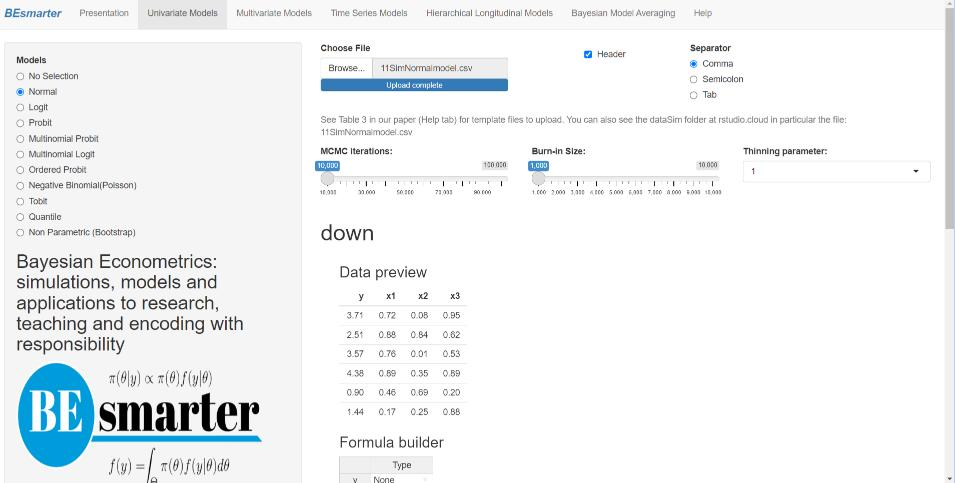
\includegraphics[width=340pt, height=130pt]{Chapters/chapterGUI/figures/Figure2.jpg}
	%%\centerline{\epsfig{/Chapters/chapter1/figures/cat.eps,width=.8\textheight,height=.4\textwidth}}
	\caption[List of figure caption goes here]{Univariate models: Specification.}\label{fig62}
\end{figure}

Then, the right-hand panel displays a widget for uploading the input dataset, which must be a \textit{csv} file with headers in the first row. Users must also select the separator type used in the input file: comma, semicolon, or tab (use the \textbf{DataSim} and \textbf{DataApp} folders for input file templates). Once the dataset is uploaded, users can preview the data. Range sliders allow users to set the number of iterations for the Markov Chain Monte Carlo algorithm, specify the burn-in period, and adjust the thinning parameter (see the following chapters in this section for technical details).

Next, users must specify the equation. This can be done using the formula builder, where they select the dependent variable and independent variables, then click on the \textit{Build Formula} tab. The equation appears in the \textit{Main Equation} space, formatted according to \textbf{R} syntax (see the main equation box in Figure \ref{fig62}, e.g., $y\sim x1+x2+x3$). Users can modify this as needed, including higher-order terms, interaction effects, or other transformations. These modifications must follow the standard formula syntax.\footnote{See \textbf{https://www.rdocumentation.org/packages/stats/versions/3.6.2/topics/formula}}

By default, univariate models include an intercept, except for ordered probit models, where the specification must explicitly exclude it due to \textit{identification} constraints (see details below).\footnote{An \textit{identification} issue arises when multiple sets of model parameters yield the same likelihood function value.} Thus, users should specify this explicitly as follows: $y\sim x1+x2+x3-1$.

Finally, users must define the prior hyperparameters. For example, in the normal-inverse gamma model, these include the mean vector, covariance matrix, shape parameter, and scale parameter (see Figure \ref{fig63}). However, our GUI uses \textit{non-informative} hyperparameters by default across all modeling frameworks, so this step is optional.

\begin{figure}
	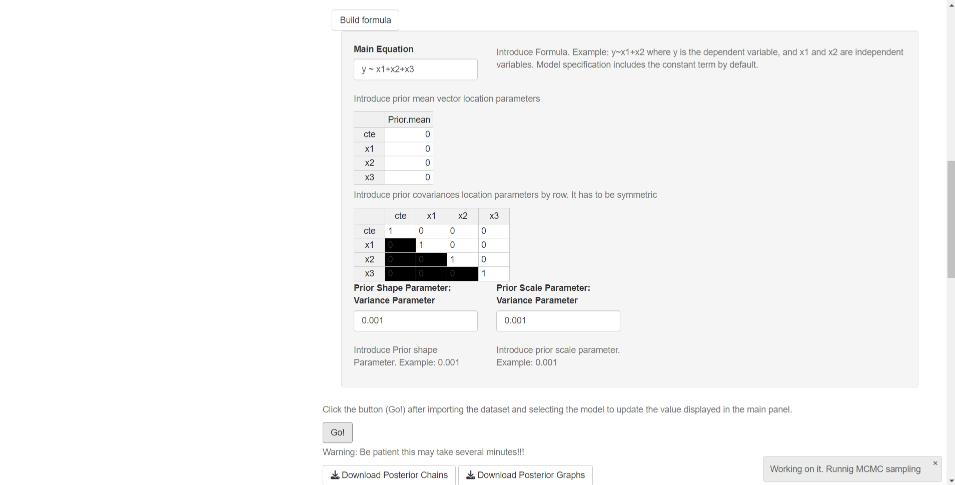
\includegraphics[width=340pt, height=130pt]{Chapters/chapterGUI/figures/Figure3.jpg}
	%%\centerline{\epsfig{/Chapters/chapter1/figures/cat.eps,width=.8\textheight,height=.4\textwidth}}
	\caption[List of figure caption goes here]{Univariate models: Results.}\label{fig63}
\end{figure}

After completing the specification process, users should click the \textit{Go!} button to initiate the estimation. Once the process is finished, our GUI displays the summary statistics and convergence diagnostics (see Figure \ref{fig63}). Additionally, widgets allow users to download the posterior chains (\textit{csv} file) and graphs (\textit{pdf} and \textit{eps} files). Note that in the results—summary, posterior chains, and graphs—the coefficients are ordered with location parameters appearing first, followed by scale parameters.

For multinomial models (probit and logit), the dataset must be structured as follows: the first column should contain the dependent variable, followed by alternative-specific regressors (e.g., alternatives' prices), and finally, non-alternative-specific regressors (e.g., income). The formula builder allows users to specify the dependent variable as well as both types of independent variables (see technical details in the next chapter). Additionally, users must define the base category, the number of alternatives (which is also required for ordered probit), the number of alternative-specific regressors, and the number of non-alternative-specific regressors (see Figure \ref{fig64}).

For multinomial logit models, users can also specify a tuning parameter—the degrees of freedom for the Metropolis–Hastings algorithm (see technical details in the next chapter). This tuning option is available in our GUI when estimation relies on the Metropolis–Hastings algorithm.

In the results of these models, coefficients are ordered as follows:

\begin{enumerate}
	\item Intercepts (\textit{cte}$_l$ in the summary display, where $l$ represents the alternative).
	\item Non-alternative-specific regressors (\textit{NAS}$_{jl}$ in the summary display, where $l$ represents the alternative and $j$ the non-alternative regressor).
	\item Alternative-specific regressors (\textit{AS}$_{j}$ in the summary display, where $j$ represents the alternative-specific regressor).
\end{enumerate}

Note that the non-alternative-specific regressors associated with the base category are set to zero and do not appear in the results. Additionally, due to identification constraints in multinomial and multivariate probit models, some coefficients in the main diagonal of the covariance matrix remain constant.

\begin{figure}
	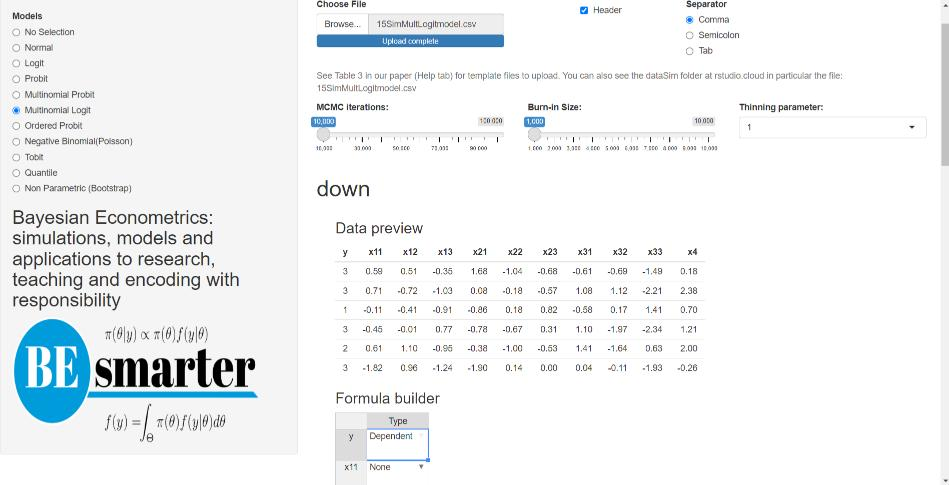
\includegraphics[width=340pt, height=130pt]{Chapters/chapterGUI/figures/Figure4.jpg}
	%%\centerline{\epsfig{/Chapters/chapter1/figures/cat.eps,width=.8\textheight,height=.4\textwidth}}
	\caption[List of figure caption goes here]{Univariate models: Multinomial.}\label{fig64}
\end{figure}

For the negative binomial model, users must specify a dispersion parameter (see the next chapter for details). Similarly, for Tobit and quantile models, users need to define the censorship points and quantiles, respectively.

The Bayesian bootstrap method only requires uploading a dataset, specifying the number of MCMC iterations, setting the resampling size, and defining the equation (see Figure \ref{fig65}). The input file should follow the same structure as the one used for the univariate normal model.

\begin{figure}
	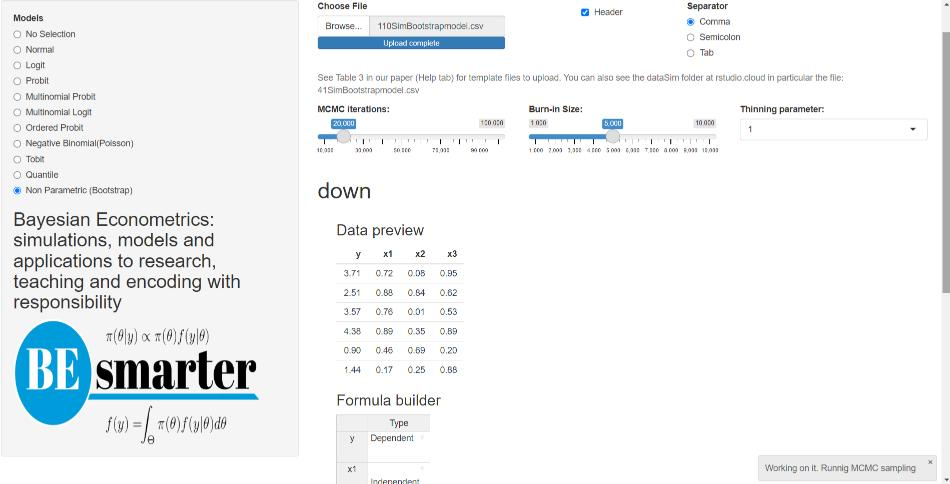
\includegraphics[width=340pt, height=130pt]{Chapters/chapterGUI/figures/Figure5.jpg}
	%%\centerline{\epsfig{/Chapters/chapter1/figures/cat.eps,width=.8\textheight,height=.4\textwidth}}
	\caption[List of figure caption goes here]{Univariate models: Bootstrap.}\label{fig65}
\end{figure}  

\section{Multivariate models}\label{secGUI3}
After our GUI is deployed (see Figure \ref{fig61}), the user should select \textit{Multivariate Models} from the top panel. Figure \ref{fig66} will then be displayed, showing a radio button on the left-hand side that lists the specific models within this category.

Figure \ref{fig66} illustrates the multivariate regression setup. The input file should first contain the dependent variables, followed by the regressors. If each equation includes an intercept, a column of 1s should be added after the dependent variables in the input file. Users can preview the data after uploading the file.

The user must specify the number of dependent variables and regressors, indicate whether an intercept should be included, and define the hyperparameter values (see Figure \ref{fig66}).

\begin{figure}
	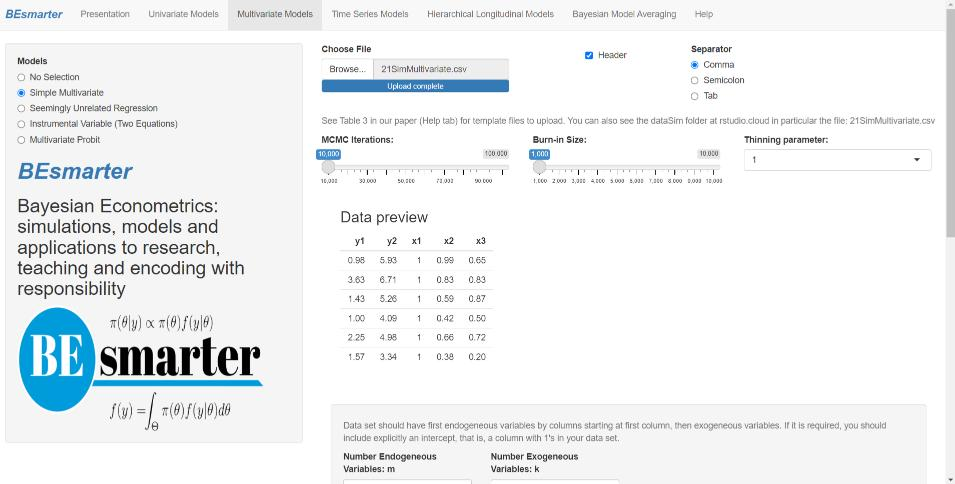
\includegraphics[width=340pt, height=130pt]{Chapters/chapterGUI/figures/Figure6.jpg}
	%%\centerline{\epsfig{/Chapters/chapter1/figures/cat.eps,width=.8\textheight,height=.4\textwidth}}
	\caption[List of figure caption goes here]{Multivariate models: Simple multivariate.}\label{fig66}
\end{figure}

In seemingly unrelated regressions, the input file should first contain the dependent variables, followed by the regressors for each equation, including the intercept (a column of 1s) if necessary. Users must define the number of dependent variables (equations), the total number of regressors (the sum of all regressors associated with the equations), and the number of regressors per equation (including the intercept if necessary). Users can also specify the values of the hyperparameters if prior information is available.

The results of the simple multivariate and seemingly unrelated regressions first display the posterior location parameters by equation, followed by the posterior covariance matrix.

In the instrumental variable setting, users should specify the main equation and the instrumental equation. This setting includes intercepts by default. The first variable on the right-hand side of the main equation must be the variable with endogeneity issues. In the instrumental equation, the dependent variable is the one with endogeneity issues, modeled as a function of the instruments. Users can also specify the values of the hyperparameters if they have prior information. The input file should include the dependent variable, the endogenous regressor, the instruments, and the exogenous regressors. The results first list the posterior estimates of the endogenous regressor, followed by the location parameters of the auxiliary regression (instrumental equation), the location parameters of the exogenous regressors, and finally, the posterior covariance matrix.

\begin{figure}
	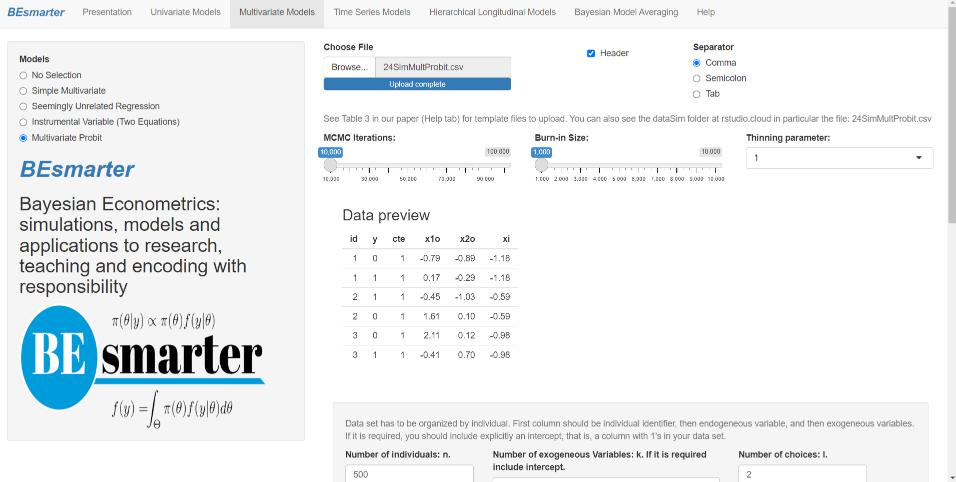
\includegraphics[width=340pt, height=130pt]{Chapters/chapterGUI/figures/Figure7.jpg}
	%%\centerline{\epsfig{/Chapters/chapter1/figures/cat.eps,width=.8\textheight,height=.4\textwidth}}
	\caption[List of figure caption goes here]{Multivariate models: Multivariate probit.}\label{fig67}
\end{figure} 

The multivariate probit model requires the input dataset to be ordered by unit. For example, three choices imply repeating each unit three times. The first column must contain the identification for each unit, using ordered integers. Next, the dependent variable should be a single vector of 0s and 1s, followed by the regressors, which must include a column of 1s for the intercepts. Users should specify the number of units, the number of regressors, and the number of choices (see Figure \ref{fig67}). The results first display the posterior location parameters by equation, followed by the posterior covariance matrix.

\section{Time series models}\label{secGUI4}
After our GUI is deployed (see Figure \ref{fig8a}), the user should select \textit{Time Series Models} from the top panel. Then, Figure \ref{fig8a} will be displayed, and the user will see the radio button on the left-hand side, which shows the specific models within this general class.

\begin{figure}
	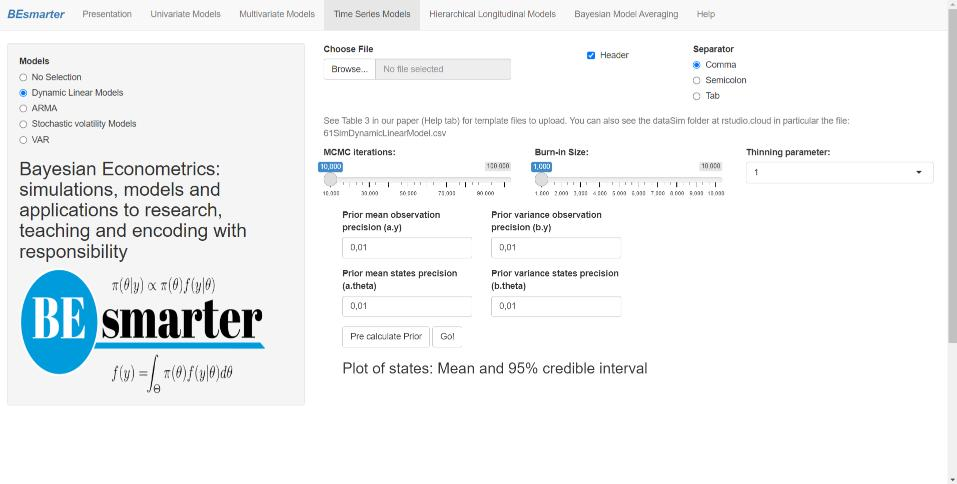
\includegraphics[width=340pt, height=130pt]{Chapters/chapterGUI/figures/Figure8a.jpg}
	%%\centerline{\epsfig{/Chapters/chapter1/figures/cat.eps,width=.8\textheight,height=.4\textwidth}}
	\caption[List of figure caption goes here]{Time series models.}\label{fig8a}
\end{figure} 

Users can perform inference using dynamic linear models (DLM), autoregressive moving average (ARMA) models, stochastic volatility models (SVM), and vector autoregressive (VAR) models. Users should upload a dataset, which must be a \textit{csv} file with headers in the first row. The files for DLMs and SVMs have the same structure: the first column contains the dependent variable, followed by the independent variables. For ARMA models, there is only one column with the modeled variable, while VAR models have each modeled variable in a separate column. Note that this version of the GUI does not allow for exogenous variables in VAR models. Users should specify the separator used in the input file: comma, semicolon, or tab. A dataset preview is displayed once the file is uploaded. Dataset templates can be found in the folders \textbf{DataSim} (see Table \ref{tab:simdata} for details) and \textbf{DataApp} (see Table \ref{tab:appdata} for details) in our \textit{GitHub} repository.

Next, users should set the MCMC and burn-in iterations using the range sliders and the thinning parameter using the input box.

To estimate DLMs, users should set the hyperparameters for the precision of the observation equation and the state equations (means and variances) if prior information is available. Otherwise, users can click the \textit{Pre Calculate Prior} button, where these hyperparameters are estimated based on a recursive model estimation using ordinary least squares (OLS). The sample size is progressively increased, and the location parameters are saved. The GUI then computes the covariance matrix of this sequence and uses it to set the prior mean for the precision of the state vector, which is equal to the inverse of the maximum element on the main diagonal of the covariance matrix ($a.theta$). The prior variance is set to ten times this value ($b.theta$). For the observation equation, the prior mean of the precision is set to the inverse of the OLS variance estimate ($a.y$), and the prior variance is set to ten times this value ($b.y$). This is a rudimentary approach to setting these hyperparameters, and users are encouraged to use a more thoughtful process.

Next, users should click the \textit{Go!} button to start estimating the model. This may take a few minutes, as DLMs are complex to estimate. Users should be patient. Once the estimation is complete, the GUI will display graphs of the states (mean and 95\% credible intervals), summary statistics of the posterior chains for the observation and state variances, and convergence diagnostics. Users can download the mean and the lower and upper limits of the 95\% credible intervals of the states, as well as the posterior chains for the variances.

For ARMA models, users need to set the frequency (annual -1-, quarterly -4-, and monthly -12-), as well as the AR and MA orders (see Figure \ref{fig8b}). Then, users should set the location and scale hyperparameters for the intercept, autoregressive (AR), moving average (MA), and standard deviation terms. Note that there is only one set of hyperparameters for the AR and MA coefficients. This step is optional, as the GUI uses non-informative priors by default.

\begin{figure}
	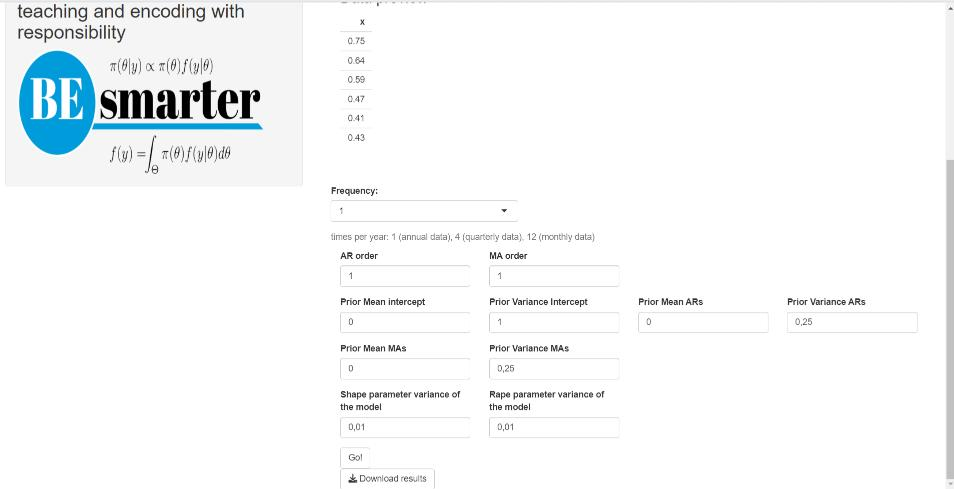
\includegraphics[width=340pt, height=130pt]{Chapters/chapterGUI/figures/Figure8b.jpg}
	%%\centerline{\epsfig{/Chapters/chapter1/figures/cat.eps,width=.8\textheight,height=.4\textwidth}}
	\caption[List of figure caption goes here]{Time series models: ARMA specification}\label{fig8b}
\end{figure}

Then, users should click the \textit{Go!} button, and the GUI will start estimating the model. The GUI will display the summary statistics of the posterior draws and the convergence diagnostics. The order is AR coefficients (if any), MA coefficients (if any), intercept, and standard deviation. Users can download the posterior chains and figures (density, autocorrelation, and trace plots).

Estimation of the SVMs requires setting the coefficients of the mean and standard deviation of the Gaussian prior for the regression parameters, the mean and standard deviation for the Gaussian prior distribution of the level of the log-volatility, shape parameters for the Beta prior distribution of the transformed persistence parameter, and a positive real number representing the scaling of the transformed volatility of log-volatility. However, this step is not necessary, as by default our GUI uses the default values in the \textit{stochvol} package.

Then, click the \textit{Go!} button, wait for the estimation to be completed, and the GUI will display the stochastic volatility plot (mean and 95\% credible interval). Users can also view the summary and diagnostics of the posterior chains (see Figure \ref{fig8c}). In addition, users can download the mean and the lower and upper limits of the 95\% credible intervals of the stochastic volatility, as well as the posterior chains of the variances.

\begin{figure}
	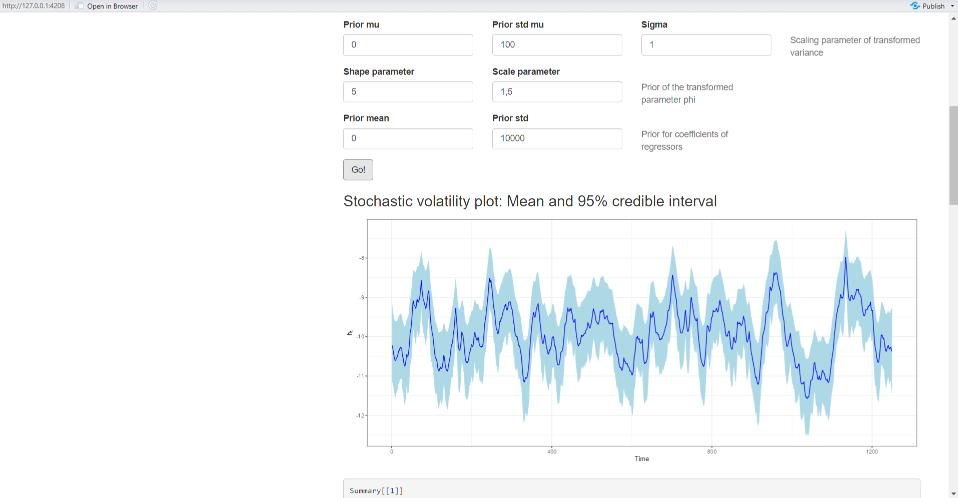
\includegraphics[width=340pt, height=130pt]{Chapters/chapterGUI/figures/Figure8c.jpg}
	%%\centerline{\epsfig{/Chapters/chapter1/figures/cat.eps,width=.8\textheight,height=.4\textwidth}}
	\caption[List of figure caption goes here]{Time series models: Stochastic volatility results.}\label{fig8c}
\end{figure} 

To estimate VAR models, users should set the number of lags, the impulse response and forecast periods, the three coefficients of the Minnesota prior, and the type of impulse response (\textit{forecast error impulse response} -feir- or \textit{orthogonalized impulse response} -other-, both cumulative or non-cumulative). See Chapter \ref{chap8} for details, Section \ref{sec84}.

Click the \textit{Go!} button, and after a few minutes, users will be able to see the plots of the impulse responses and forecasts (means and 95\% credible intervals). Click the \textit{Download Results} button, and a zip file with \textit{.csv} files containing the impulse responses and forecasts, along with their plots, will be downloaded.

\section{Longitudinal/panel models}\label{secGUI5}
After our GUI is deployed (see Figure \ref{fig61}), the user should select \textit{Hierarchical Longitudinal Models} in the top panel. Then, Figure \ref{fig68} will be displayed, and the user can see the radio button on the left-hand side that shows the specific models inside this generic class.

The hierarchical longitudinal models tab allows for estimating models that account for within-subject correlation when the dependent variable is continuous (Normal), binary (Logit), or a count (Poisson).

The input files for hierarchical longitudinal models should first include the dependent variable, followed by the regressors and a cross-sectional identifier ($i=1,2,\dots,N$). It is not a requirement to have a balanced dataset: $T_i$ can be different for each $i$ (see Chapter \ref{chap9} for technical details). Users can see templates of datasets in the folders \textbf{DataSim} (see Table \ref{tab:simdata} for details) and \textbf{DataApp} (see Table \ref{tab:appdata} for details) in our \textit{GitHub} repository. When the dataset is uploaded, users will have a preview of it.

Users should also specify the fixed part equation and the random part equation, both in \textbf{R} format. If only random intercepts are required, do not enter anything in the latter part (see Figure \ref{fig68}). Users should also type the name of the cross-sectional identifier variable. The results displayed and the posterior graphs are associated with the fixed effects and covariance matrix. However, users can download the posterior chains of all posterior estimates: fixed and random effects, and the covariance matrix.

\begin{figure}
	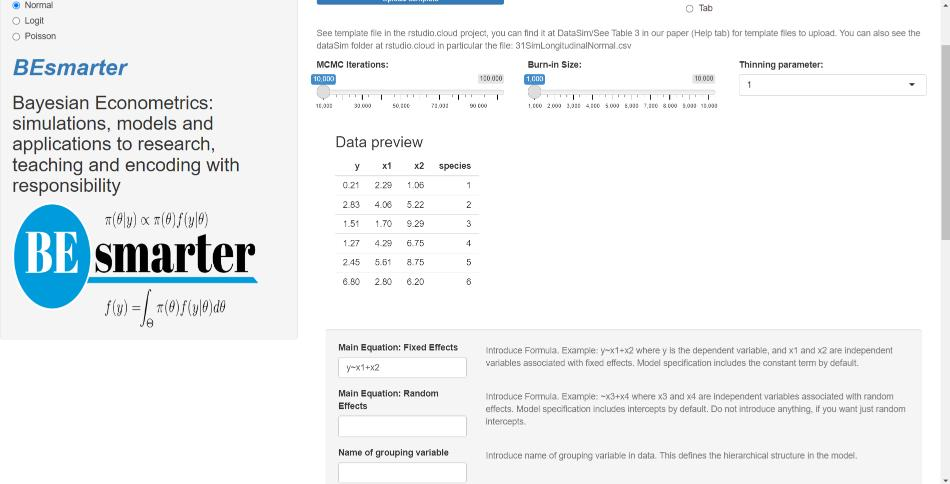
\includegraphics[width=340pt, height=130pt]{Chapters/chapterGUI/figures/Figure8.jpg}
	%%\centerline{\epsfig{/Chapters/chapter1/figures/cat.eps,width=.8\textheight,height=.4\textwidth}}
	\caption[List of figure caption goes here]{Hierarchical longitudinal models: Specification.}\label{fig68}
\end{figure} 

\section{Bayesian model average}\label{secGUI6}

After our GUI is deployed (see Figure \ref{fig61}), the user should select \textit{Bayesian Model Averaging} in the top panel. Then, Figure \ref{fig69} will be displayed, and the user can see the radio button on the left-hand side that shows the specific models inside this generic class.

Bayesian model averaging (BMA) based on a Gaussian distribution can be carried out using the Bayesian information criterion (BIC) approximation, Markov chain Monte Carlo model composition (MC3), instrumental variables (see Figure \ref{fig69}), and dynamic BMA. The first two approaches require an input dataset where the first column is the dependent variable, followed by the potentially important regressors.

Users should set the bandwidth model selection parameter ($O_R$) and the number of iterations for BIC and MC3, respectively (see Chapter \ref{chap10} for technical details). The results include the posterior inclusion probability ($p \neq 0$), expected value (EV), and standard deviation (SD) of the coefficients associated with each regressor. The BIC framework also displays the most relevant models with their posterior model probabilities (PMP). Users can download two \textit{csv} files: \textit{Best models} and \textit{Descriptive statistics coefficients}. The former is a 0-1 matrix such that the columns are the regressors and the rows are the models; a 1 indicates the presence of a specific regressor in a specific model, and 0 indicates its absence. Note that the last column of this file is the posterior model probability for each model (row). The latter file shows the posterior inclusion probabilities, expected values, and standard deviations associated with each regressor, taking into account the BMA procedure based on the best models.

\begin{figure}
	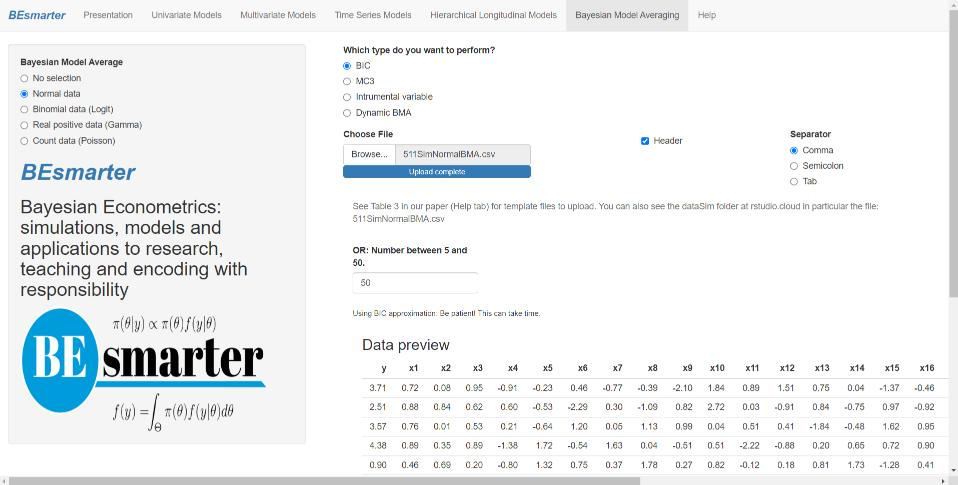
\includegraphics[width=340pt, height=130pt]{Chapters/chapterGUI/figures/Figure9.jpg}
	%%\centerline{\epsfig{/Chapters/chapter1/figures/cat.eps,width=.8\textheight,height=.4\textwidth}}
	\caption[List of figure caption goes here]{Bayesian model averaging: Specification and results.}\label{fig69}
\end{figure} 

Bayesian model averaging with endogeneity issues requires two input files. The first file should have the dependent variable in the first column, followed by the regressors with endogeneity issues, and then the exogenous regressors. The user should include a column of 1's if an intercept is required. The second input file contains all the instruments. Users should also specify the number of regressors with endogeneity issues (see Figure \ref{fig610}).

\begin{figure}
	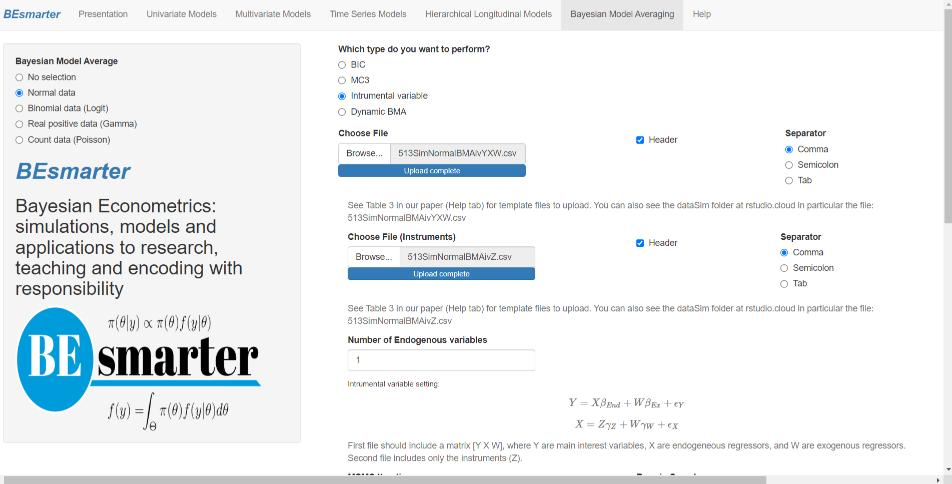
\includegraphics[width=340pt, height=130pt]{Chapters/chapterGUI/figures/Figure10.jpg}
	%%\centerline{\epsfig{/Chapters/chapter1/figures/cat.eps,width=.8\textheight,height=.4\textwidth}}
	\caption[List of figure caption goes here]{Bayesian model averaging: Instrumental variable specification.}\label{fig610}
\end{figure} 

The results include the posterior inclusion probabilities and expected values for each regressor. The user can find the results of the main equation, and then of the auxiliary equations. Users can download \textit{csv} files of BMA results for both the second stage (main equation) and the first stage (auxiliary equations). In addition, users can download the posterior chains of the location parameters of the main equation, $\beta_{l}$, $l=1,2,\dots,dim\left\{\bm{\beta}\right\}$, the location parameters of the auxiliary equations, $\gamma_{j,i}$, $j=1,2,\dots,dim\left\{\bm{\beta}_s\right\}$ where $dim\left\{\bm{\beta}_s\right\}$ is the number of regressors with endogeneity issues, $i=1,2,\dots,dim\left\{\bm{\gamma}\right\}$, where $dim\left\{\bm{\gamma}\right\}$ is the number of regressors in the auxiliary regressors (exogeneous regressors + instruments), and the elements of the covariance matrix $\sigma_{j,k}$ (see Chapter \ref{chap10} for technical details).

Dynamic BMA also requires two files. The first is the dataset with the dependent variable and potential regressors, and the second file describes the competing models. There is one column for each regressor and one row for each competing model; 0 indicates that the regressor is not in the model, and 1 indicates that it is in the model. Users can see templates of this file in the folders \textbf{DataSim} (see Table \ref{tab:simdata} for details) and \textbf{DataApp} (see Table \ref{tab:appdata} for details) of our \textit{GitHub} repository.

Then, the users should set the \textit{forgetting parameters} of the covariance and transition matrices and click the \textit{Go!} button. A plot of the PMPs of the competing models is displayed, and users can click the \textit{Download the results for DBMA}. Two files are downloaded: the first contains the dynamic Bayesian average filtering recursions for each state, and the second contains the PMP of each model and the dynamic Bayesian model averaging prediction.

Bayesian model averaging based on BIC approximation for non-linear models (Logit, Gamma, and Poisson) requires an input dataset where the first column is the dependent variable, and the other columns are the potentially relevant regressors. Users should specify the bandwidth model selection parameters, also referred to as Occam's window parameters ($O_R$ and $O_L$). Our GUI displays the posterior inclusion probabilities ($p!=0$), the expected value of the posterior coefficients (EV), and the standard deviation (SD). In addition, users can view the results associated with the models with the highest posterior model probabilities and download \textit{csv} files with the results of specifications of the best models and descriptive statistics of the posterior coefficients from the BMA procedure. These files are similar to the results of the BIC approximation for the Gaussian model.

\section{Help}\label{secGUI7}

The last tab in our GUI is \textit{Help}. There, you can find the \textit{PDF} version of this book and the link to the \textit{HTML} online version. Users can also send me an email at \textit{aramir21@gmail.com} for any questions, comments, or suggestions.

\section{Warning}\label{secGUI8}

Users should also note that sometimes our GUI shuts down. In our experience, this is due to computational issues arising from the implicit commands we call when estimating certain models. These issues may include computationally singular systems, missing values where TRUE/FALSE are needed, L-BFGS-B requiring finite values for ``fn'', NA/NaN/Inf values, or errors in \texttt{backsolve}. These issues can sometimes be resolved by adjusting the dataset, such as avoiding high levels of multicollinearity.

It should also be noted that when warning messages are displayed in our GUI, there is a high likelihood of convergence issues with the posterior chains. Therefore, the results may not be trustworthy. Users can identify these problems by checking the console in their \textit{RStudio} sections, where the specific folder/file where the issue occurred will be specified. In any case, we would appreciate your feedback to improve and enhance our GUI.

We should also mention that there are many ways to improve the codes presented in this book, and particularly, the following five chapters. For instance, the \textit{MCMCpack} and \textit{bayesm} packages perform most of the matrix operations in C++ using the \textit{Rcpp} package. This substantially speeds up the algorithms compared to the codes presented in the next chapters when we program from scratch the samplers. We could further improve the computational times of our codes using parallel computing and the \textit{Rcpp} package, but this requires more advanced skills that are not covered in this book.